%
% 01_NWP.tex -- Beispiel-File für das Paper
%
% (c) 2023 Prof Dr Andreas Müller, OST Ostschweizer Fachhochschule
%
% !TEX root = ../../buch.tex
% !TEX encoding = UTF-8
%
\section{Numerische Wettervorhersage
\label{spektral:section:nwp}}
\rhead{Numerische Wettervorhersage}

\subsection{Finite-Difference-Gittermodelle
\label{spektral:subsection:gittermodelle}}
In den meisten Fällen ist die Lösung von partiellen Differentialgleichungen nur mithilfe von numerischen iterativen Methoden möglich. 
Die Idee dieser Methoden besteht darin, die Differentialgleichungen zu diskretisieren.
Die Ableitungen werden durch finite Differenzen dargestellt.
Dadurch können die Differentialgleichungen in algebraische Gleichungssysteme umgewandelt werden.
D.h. es werden die Werte der Variablen nicht für die gesamte unendliche Menge von Punkten im Bereich untersucht, sondern nur für eine endliche Teilmenge.

Die Methode der endlichen Differenzen beinhaltet die Diskretisierung von Funktionen auf einem Gitter.
In diesem Fall sind die Werte der Funktion die Knoten des Gitters und Ableitungen werden durch endliche Differenzen ersetzt.

Vorwärtsdifferenz:
\begin{equation}
\frac{\mathrm{d}u}{\mathrm{d}t} = \frac{u(t + \Delta{t}) - u(t)}{\Delta{t}}
\label{spektral:equation1}
\end{equation}

Rückwärtsdifferenz:
\begin{equation}
\frac{\mathrm{d}u}{\mathrm{d}t} = \frac{u(t) - u(t - \Delta{t})}{\Delta{t}}
\label{spektral:equation2}
\end{equation}

Zentraledifferenz
\begin{equation}
\frac{\mathrm{d}u}{\mathrm{d}t} = \frac{u(t + \Delta{t}) - u(t - \Delta{t})}{2\Delta{t}}
\label{spektral:equation3}
\end{equation}

Üblicherweise werden Diskretisierungsgitter gewählt, die mit den Koordinatengittern übereinstimmen.
In einem zweidimensionalen kartesischen Koordinatensystem stellen die Gitterzellen die Rechtecke dar.
\pagebreak
\begin{figure}[h]
	\centering
	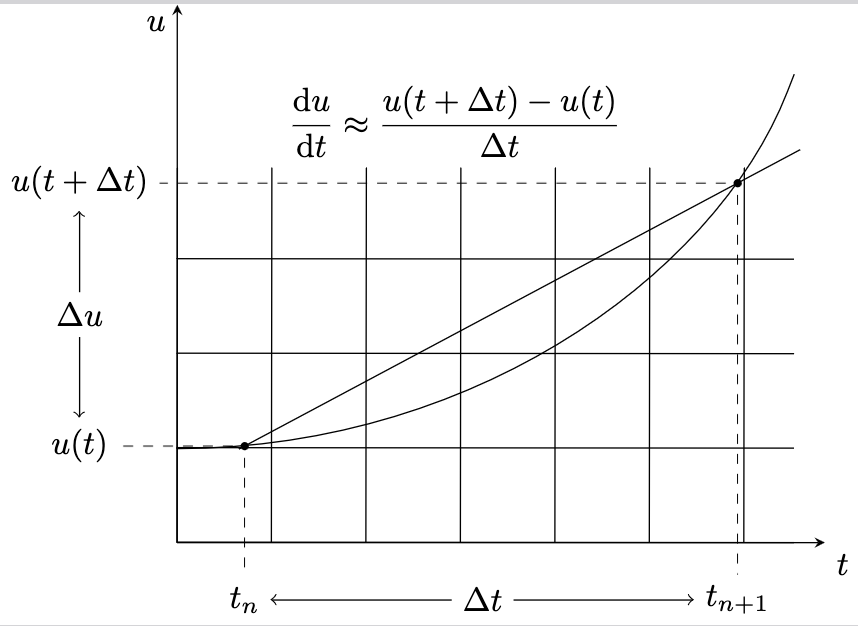
\includegraphics[height=120pt]{papers/spektral/images/forwarddiff.png}
	\caption{Vorwartsdifferenz}
    \label{spektral:fig:gittermodelle}
\end{figure}

Auf der Abbildung 16.1 sieht man, dass für eine 1d-Funktion werden viele Punkte für die Vorheraussage benötigt. In der 3-Dimensionen es sind die Millionen von Datenpunkten und, damit man eine gute Wetterprognose mit der Methode machen kann, werden höhe Rechnungsleistungen benötigt.

Ein Optimierung ist, die Prognosenfunktion auf eine andere Art zu aproximieren.


\subsection{Was sind die spektrale Modelle?
\label{spektral:subsection:spektralemodelle}}
In den 1980er Jahren des 20. Jahrhunderts wurden neben den gitterbasierten (Finite-Difference) Lösungsmethoden, die traditionell in Vorhersagemodellen verwendet wurden, auch Methoden angewendet, bei denen die räumliche Abhängigkeit der prognostizierten meteorologischen Werten als Reihen von Funktionssystemen dargestellt wird, die bestimmte Eigenschaften aufweisen.

In diesem Fall wird die prognostizierte Gleichung oder das System von partiellen Differentialgleichungen auf Systeme von Differentialgleichungen für die zeitabhängigen Koeffizienten der Zerlegung reduziert.
Die gesuchte Werte bei diesem Ansatz sind diese Koeffizienten und nicht die Werte der prognostizierten Funktionen an den Gitterpunkten. 
Eine Variante dieser Methode im Bereich der numerischen Wettervorhersage wird als spektrale Methode bezeichnet und Vorhersagemodelle, bei denen die Gleichungen mit der spektralen Methode gelöst werden, werden als spektrale Modelle bezeichnet.

Spektrale Modelle sind eine Art numerischer Modelle, die in verschiedenen wissenschaftlichen Bereichen, einschließlich der Meteorologie, verwendet werden.
Diese Modelle basieren auf der Verwendung spektraler Methoden, um mathematische Gleichungen, die physikalische Phänomene beschreiben, zu lösen.

In der Meteorologie beziehen sich spektrale Modelle auf Vorhersagemodelle, die spektrale Methoden verwenden, um atmosphärische Prozesse zu simulieren und Wettervorhersagen zu erstellen.
Anstatt die Erde und die Atmosphäre in einem diskreten Gitter zu modellieren, wie es bei gitterbasierten Modellen der Fall ist, verwenden spektrale Modelle eine Fourier-Transformation, um die Atmosphäre in eine Kombination von Wellen mit verschiedenen Frequenzen aufzubrechen.
Dies ermöglicht es, die Atmosphäre kontinuierlich und mit höherer Auflösung zu modellieren.

Insgesamt sind spektrale Modelle ein wichtiger Ansatz, um detaillierte Einblicke in atmosphärische Prozesse zu gewinnen und präzise Wettervorhersagen zu erstellen, insbesondere wenn es um die Wellen und die Schwingungen geht.

\subsection{Kugelkoordinaten
\label{spektral:subsection:kugelkoordinaten}}

Bevor wir die spektrale Modelle nähe anschauen, müssen wir die von den kartesischen Koordinaten zu den Kugelkkordinaten wecheln, weil wir uns auf einer Kugel befinden. Siehe Abbildung 16.2

\begin{wrapfigure}{r}{0.25\textwidth}
	\centering
	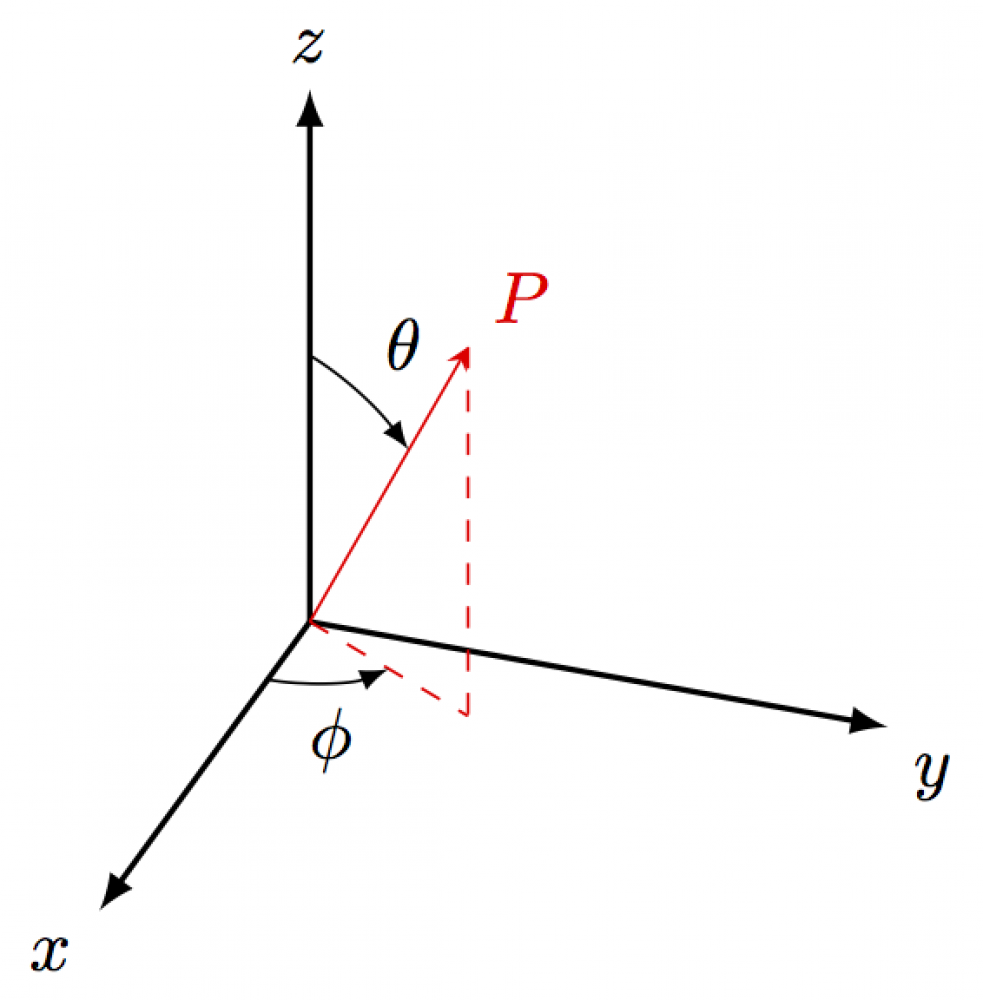
\includegraphics[height=120pt,width=120pt]{papers/spektral/images/spherical_coordinates.png}
	\caption{Sphärische Koordinaten}
    \label{spektral:fig:sphericalcoords}
\end{wrapfigure}

\begin{equation}
 x = r*sin(\theta)*cos(\phi)
\label{spektral:equation4}
\end{equation}

\begin{equation}
 y = r*sin(\theta)*sin(\phi)
\label{spektral:equation5}
\end{equation}

\begin{equation}
 z = r*cos(\theta)
\label{spektral:equation6}
\end{equation}

wobei |r| > 0 sein muss, sonst können $\theta$ und $\phi$ nicht definiert werden.


